% !TEX root = ../SEM-ReadMe.tex
%% -----------------------------
%% Stand: 2022/10/10
%% -----------------------------
\section{Einige Empfehlungen}
\subsection{Eingabe des Textes}
%
Da in der Regel ein deutscher Text eingegeben wird, müssen auch die Regeln der deutschen Rechtschreibung und Zeichensetzung beachtet werden.
Dies wir mit dem Paket \texttt{babel} \cite{babel} erreicht:

\begin{enumerate}
\item
Richtige \enquote{Gänsefüßchen} mittels \verb|\enquote{...}|.

\item
Richtige Trennung, auch für das Wort \emph{Urinstinkt}.

\item
Richtige Eingabe von: siehe etwa \og oder \dh oder \etc \ldots
\end{enumerate}
%
Dies erreicht man mittels 
%\usepackage[babel,german=guillemets]{csquotes}
%\babelprovide[hyphenrules=ngerman-x-latest]{ngerman}
%
%\begin{tcolorbox}%lstlisting}{listing only}
%\cs{usepackage[ngerman]\brackets{babel}}
%\end{tcolorbox}
%
\begin{tcblisting}{listing only}
\documentclass[ngerman]{scrartcl}
\usepackage[ngerman]{babel}
\usepackage[austostyle,german=guillemets]{csquotes}
\babelprovide[hyphenrules=ngerman-x-latest]{ngerman}
...
\begin{document}
...
\end{document}
\end{tcblisting}
%%
Also etwa
%
\begin{tcblisting}{title= \enquote{Anführungszeichen Deutsch}}
Richtig: \enquote{Gänsefüßchen}
Und noch richtiger: \enquote{Gänsefüßchen und nochmals \enquote{Gänsefüßchen} im Text}
\end{tcblisting}
%
%In beiden Fällen kann man in eine andere Sprache umschalten, etwa von deutsch auf englisch:
%%
%\begin{tcblisting}{title= \enquote{Anführungszeichen Englisch}}
%\begin{otherlanguage}{english}
%Now we get \enquote{the right one.}
%Additionally: \enquote{Gänsefüßchen and once more \enquote{Gänsefüßchen} in the text.}
%\end{otherlanguage}
%\end{tcblisting}
%
Wer aber weitere Sprachen nutzen will, muss dieses entsprechend ergänzen.
Details hierzu und wie man umschaltet findet man im Manual zum Paket \lpkg{babel} unter 
\href{https://ctan.ebinger.cc/tex-archive/macros/latex/required/babel/base/babel.pdf}{babel.pdf} oder man schaut mal in \textcite[3.7.2]{voss:2012a} rein.
%
\subsection{Eingabe von Mathematik}\label{subsec:eingabe-mathe}
Einer der Stärken von \TeX{} ist die Eingabe mathematischer Ausdrücke, wie etwa
%
\[
	\frac{ a+b }{ c+ \frac{ 1 }{ d+e } }
\]
%
oder von mathematischen Umgebungen, wie etwa so:
%
\begin{theorem}\label{thm:hauptsatz}
%	
Ist $ f $ eine stetige reellwertige Funktion auf dem Intervall\/ $ \interval{0,1} $, so ist
%
\[
  	F( t ) = \int_{ 0 }^{ t } f(s) \ds
\]
%
differenzierbar auf diesem Intervall und $ F'(t) = f(t) $ für alle $ t \in \interval{0,1} $ .
\end{theorem}
%
Vor allem kann man später immer auf dieses Theorem über Querverweise einfach zurückgreifen, also \enquote{siehe \cref{thm:hauptsatz}} funktioniert (wenn man alles richtig gemacht hat).
Basis dazu ist das Paket \texttt{amsmath}, eine Entwicklung der American Mathematical Society \href{https://de.wikipedia.org/wiki/American_Mathematical_Society}{AMS}.

Auch hier, mehr noch als bei der Eingabe von reinem Text, gilt es sorgfältig zu arbeiten. 
Mein Tipp: \enquote{Platz lassen}, wie etwa bei der Eingabe des obigen Bruchs
%
	\begin{tcblisting}{title=Eingabe einer Formel, listing only}
		%
		\[
			\frac{a+b}{c + \frac{1}{d+e}}
		\]
		%
	\end{tcblisting}
%
Dies ist einfacher zu \enquote{lesen}, speziell, wenn es komplexer wird.
So sollte es jedenfalls nicht aussehen:
%
\begin{center}
	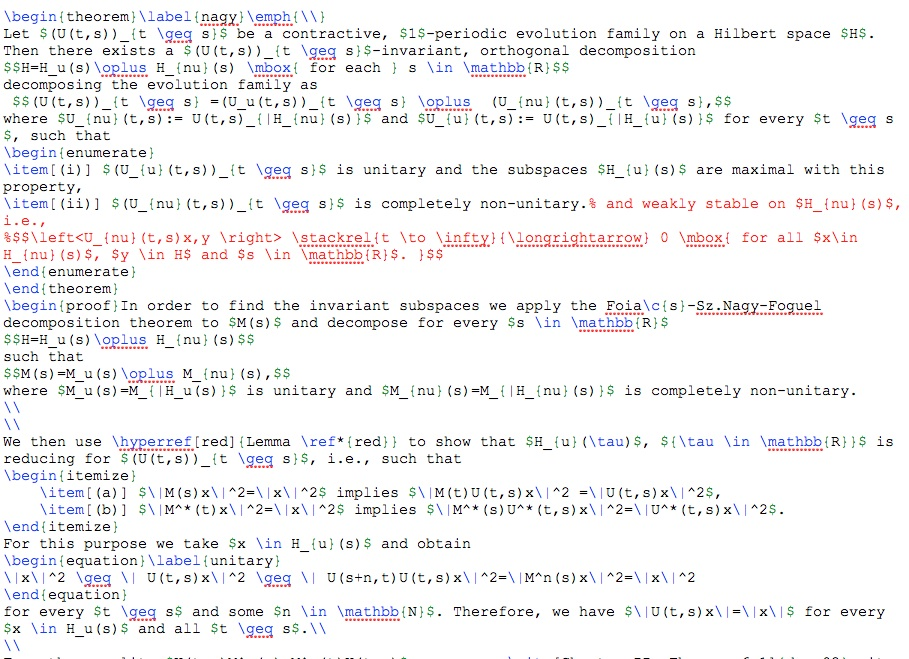
\includegraphics[scale=0.4]{./content/example2}
\end{center}
%
Am Anfang (und auch später) wird man öfters ein Buch zu Rate ziehen, wenn es um die Eingabe von speziellen Zeichen wie Integral $ \int $ oder Summen $ \sum_{ n = 1 }^{ \infty } r_{ n } $ geht.
Die Literatur und \href{http://tug.ctan.org/info/symbols/comprehensive/symbols-a4.pdf}{\LaTeX{}-Symbole} \cite{comprehensive} helfen dabei.
%Als Begleitliteratur für den mathematischen Teil empfehle ich das Buch \textcite{voss:2012b} oder \textcite{graetzer:2007}.
Ein nettes Hilfsmittel zum Üben und zum Erstellen mathematischer Formeln ist \href{https://www.chachatelier.fr/latexit/}{LaTeXit} -- leider nur für die Nutzer eines Apple Mac-Systems.

Noch ein Hinweis: Der Mathematikmodus hat zwei Varianten:
%
\begin{myitemize}
	
	\item
	Der \emph{Inline}-Modus via \verb!$ \alpha $! oder \verb|\( \alpha \)|: Beides ergibt \( \alpha \) in der Zeile (oder die Summe weiter oben).
	Ich denke, dass die Eingabe  mittels \verb|$ ... $| besser ist, da diese sich von den Klammern abhebt, die man in der Regel noch zusätzlich hat.
	
	\item
	Der \emph{abgesetzte Modus}: Siehe hierzu das Beispiel zu den Brüchen.
	Für diesen ist es \emph{verboten}, die Variante \verb!$$ ... $$! zu nutzen.
	Diese ist eine \sog Primitive aus dem Fundus von \TeX{} und schon seit den Zeiten der ersten Version von \LaTeX{} nicht mehr sinnvoll.
		
	\begin{tcblisting}{title=Abgesetzte Formel ohne Nummer}
		%
		\[
			\frac{a+b}{c + \frac{1}{d+e}}
		\]
		%
	\end{tcblisting}
	%%
		\begin{tcblisting}{title=Abgesetzte Formel mit Nummer}
		%
		\begin{equation}\label{eq:gleichung}
			\frac{a+b}{c + \frac{1}{d+e}}
		\end{equation}
		%
	\end{tcblisting}
\end{myitemize}
%%
Noch ein Hinweis, da ich dieses mehrfach gesehen habe: Die \texttt{align*}-Umgebung ist kein Ersatz für die beiden \og abgesetzten Umgebungen sondern -- wie der Name sagt.
Beispiele dazu findet man in dem bereits erwähnten AMS-Guide \cite{short-math-guide}.

%% --
Zu beachten ist auch, dass für die Eingabe eines mathematischen Textes typographische Regeln gelten.
Die wesentlichen:

\begin{myenumerate}
	\item
	Grundsätzlich kursiv werden einfache Variable $ x $, $ y $, mathematische Funktionen $ z = f(x) $ oder Indizes $ x_{ j } $ gesetzt.
	
	\item
	Aufrecht gesetzt werden alle Ziffern $ 1 23 $, mathematische Funktionen mit bestimmten Eigenschaften, etwa $  \sin(x) $, Maßeinheiten wie $ 12 \, \mathrm{kg} $ \etc

\end{myenumerate}
%
Weiteres findet sich im Detail in \textcite{voss:2012b} oder \textcite{nadler:formelsatz}.

Ein Beispiel:
%% --
\begin{tcblisting}{title = Nicht korrekt, lower separated=false}
$ ds^2=dx^2+dy^2+dz^2-c^2dt^2 $
\end{tcblisting}
%%
\vs 
%%
\begin{tcblisting}{title = Richtig, lower separated=false}
\renewcommand*{\d}[1]{\mathop{}\!\mathrm{d}{#1}}
%
$ \d{s}^{2} = \d{x}^{2} + \d{y}^{2} + \d{z}^{2} - c\d{t}^{2} $
\end{tcblisting}

%%
\subsection{Mathematische Umgebungen}
Für die Theoreme etc.\@ wird das Paket \texttt{amsthm} \cite{amsthm} verwendet.
Das Prinzip ist immer das gleiche: Man verwendet die Konstruktion der Umgebungen von \LaTeX{}{} und benennt diese.
Die Grundkonstruktion ist 
%
\begin{tcblisting}{title = Mathematische Umgebungen, listing only}
\begin{name}\label{key:kuerzel}
 ....
\end{name}
\end{tcblisting}
%
wobei mit \verb!\label{..}! ein Querverweis mit Hilfe von \verb|\ref{...}| ermöglicht wird (siehe hierzu den entsprechenden \LaTeX{}-Tipp).
%
\begin{tcblisting}{title = Ein Theorem}
\begin{theorem}
\[
 \int \ldots
\]
\end{theorem}
\end{tcblisting}
%
\begin{tcblisting}{title = Ein Korollar}
Text
%
\begin{corollary}
  Also ist \ldots
\end{corollary}
%
oder
%
\begin{cor}
  Also ist \ldots
\end{cor}
%
wer es kürzer will.
\end{tcblisting}
%
Diese Definitionen erfolgen normalerweise in der Präambel.
Da diese aber unübersichtlich wird, sind alle Definitionen in die Datei
%%
\begin{tcolorbox}
SEM-art.tex
\end{tcolorbox}
%
ausgelagert und dort -- neben anderen -- vordefiniert und können so gleich genutzt werden.
%
\begin{tcblisting}{listing only}
		\newtheorem{theorem}{Theorem}
		\newtheorem{thm}{Theorem}
		\newtheorem{corollary}[theorem]{Korollar}
		\newtheorem{cor}[theorem]{Korollar}
\end{tcblisting}
%
%und ist in unserem Fall bereits vordefiniert, siehe \vref{tab:ma-umgebungen} für die Möglichkeiten.
%In allen Editoren zur Eingabe der \TeX{}-Syntax gibt es die Möglichkeit, die Eingabeformate als Tasttaturkürzel abzulegen.
%Bitte hierzu die Dokumentation des verwendeten Editors nachlesen.
Wichtig ist es, die Umgebungen mit einem korrekten Label zu versehen, da man dann die Möglichkeit hat, einfach darauf zu verweisen.
Es sieht dann etwa so aus: \ldots der Hauptsatz (siehe \vref{thm:hauptsatz}) gibt \ldots .

Die Details hierzu sind in einigen Tipps beschrieben, den sich auf ILIAS befinden.

\subsection{Aufzählungen}
Für Aufzählungen in Theorem, Sätzen \etc -- aber nicht nur hier --  gelten grundsätzlich die folgende Regeln:
%
\begin{enumerate}[(1)]
	\item 
	Aufzählungen, die keine Äquivalenzen sind, werden grundsätzlich mit kleinen \emph{römischen} Ziffern gekennzeichnet (also (i), (ii), \dots).
Die Eingabe erfolgt mittels
%
	\begin{center}
		\begin{lstlisting}
 			\begin{enumerate}[(i)]
				\item ..
			\end{enumerate}
		\end{lstlisting}
 	\end{center}
	
	\item
	Äquivalenzen  werden grundsätzlich mit den kleinen Buchstaben gekennzeichnet, also (a), (b), \dots .
	Die Eingabe erfolgt mittels	
	%
	\begin{center}
		\begin{lstlisting}{listing only}
			\begin{enumerate}[(a)]
				\item ..
			\end{enumerate}
		\end{lstlisting}
	\end{center}
	%
	
%	\item
%	Nummerierungen (also (1), (2), \dots oder ähnliches) erfolgen mittels
%	
%	\begin{center}
%		\begin{lstlisting}
% 			\begin{enumerate}[(1)]
% 			
%				\item ..
%			\end{enumerate}
%		\end{lstlisting}
%	\end{center}
%	%
			
\end{enumerate}
%
Notwendig, damit dieses funktioniert, ist das Paket \texttt{enumitem} \cite{enumitem}, was aber geladen wird.
Wer mehr dazu wissen will, kann es sich mittels \verb!texdoc enumitem! anzeigen lassen -- oder auf \href{https://ctan.org/pkg/enumitem}{diesen Link} klicken -- in dem Musterfile ist es bereits integriert.
Ansonsten kann man dieses auch für Aufzählungen in einer normalen Textumgebung nutzen und entsprechend anpassen.
%% --
\subsection{Literaturverzeichnis}
Hier gibt es zwei Möglichkeiten: 

\begin{myitemize}

\item 
Die \enquote{normale} Variante über die in \LaTeX{} enthaltene Umgebung 
%
\begin{tcblisting}{ title=Literaturverzeichnis, listing only}
\begin{thebibliography}{99}
%
\bibitem{graetzer:2007} George Grätzer,  
\emph{More Math into \LaTeX{}}, Springer (2007)
\ldots
\end{thebibliography}
\end{tcblisting}
%
Dies findet sich in der Musterdatei als Beispiel und ist völlig ausreichend für die Arbeit im Rahmen der Hausarbeit (oder für Arbeiten mit wenig Literatur).
Bitte die Art und Weise der Eingabe von Referenzen in der Literatur, etwa in \textcite{voss:2012a} nachlesen.
	
	\item
	Für größere Literaturzitate und -Sammlungen nutzt man das Paket \texttt{biblatex}  \textcite{voss:2011}. 
	Wer wissen will, wie dies geht: Bitte in \textcite{latextipps6} reinsehen.	
\end{myitemize}
%
Nebenbei: Die Pflege einer Literaturdatenbank erfolgt entweder über \href{https://de.wikipedia.org/wiki/BibDesk}{BibDesk} für Mac-Nutzer oder sonst mit \href{https://de.wikipedia.org/wiki/JabRef}{Jabref} sonst.
Wichtig sind auch die richtigen Abkürzungen der mathematischen Reihen, bei denen ein Artikel erschienen ist.
Dabei hilft \href{https://images.webofknowledge.com/images/help/WOS/A_abrvjt.html}{diese Unterlage}.
%

\subsection{Beamer}
%\subsubsection{}
Zum Schluss noch ein Hinweis auf \href{https://de.wikipedia.org/wiki/Beamer_(LaTeX)}{Beamer}: Dies ist ein System, das auf \TeX{} und \LaTeX{} aufbaut und die Erstellung von Präsentationen ermöglicht.
Ich denke, alle kennen \emph{Powerpoint}, das aber nur bedingt im naturwissenschaftlichen Umfeld sinnvoll eigesetzt werden kann (wegen der mathematischen Ausdrücken).
Vielleicht eine Gelegenheit, im Rahmen von Vorträgen \emph{Beamer} zu probieren.

Eine kleine Vorlage ist beigefügt -- \texttt{SEM-Baemer.tex} -- und unter 
 \url{https://bit.ly/3XeXp6R} findet man eine (kleine große) Übersicht.
Darüberhinaus gibt es auch auf YouTube Einführungen dazu, übrigens auch zu \LaTeX{}.
Die Definitionen für die Vorlage finden sich unter \texttt{./preamble/Beamer-defn.tex} und können natürlich angepasst werden.
%%
